%
% $RCSfile: memory.tex,v $
%
% Copyright (C) 2002-2008. Christian Heller.
%
% Permission is granted to copy, distribute and/or modify this document
% under the terms of the GNU Free Documentation License, Version 1.1 or
% any later version published by the Free Software Foundation; with no
% Invariant Sections, with no Front-Cover Texts and with no Back-Cover
% Texts. A copy of the license is included in the section entitled
% "GNU Free Documentation License".
%
% http://www.cybop.net
% - Cybernetics Oriented Programming -
%
% http://www.resmedicinae.org
% - Information in Medicine -
%
% Version: $Revision: 1.1 $ $Date: 2008-08-19 20:41:07 $ $Author: christian $
% Authors: Christian Heller <christian.heller@tuxtax.de>
%

\subsection{Memory}
\label{memory_heading}
\index{Memory}
\index{Persistent Memory}
\index{Transient Memory}
\index{Volatile Memory}
\index{Sensory Memory}
\index{Long Term Memory}
\index{LTM}
\index{Short Term Memory}
\index{STM}
\index{Knowledge Memory}
\index{Signal Memory}
\index{Internal Memory}
\index{Input/ Output Memory}
\index{Event Queue}

The application/ domain knowledge a control software processes resides in a
\emph{Memory}. Two different kinds known from \emph{Informatics} are the
\emph{persistent} and \emph{transient} (\emph{volatile}) memory (section
\ref{persistent_and_transient_heading}). For the system architecture
investigated in this section, the term \emph{Memory} does not refer to
hardware, but to a special data structure for knowledge storage.

Section \ref{short_and_long_term_memory_heading} introduced the
\emph{Sensory Memory}, \emph{Long Term Memory} (LTM) and \emph{Short Term Memory}
(STM), so labelled by the science of psychology. Sensory memory stores data
arriving from input organs; LTM stores past contents; STM holds temporary
information to be processed within the system. A knowledge-processing system
with human archetype -- such as the one proposed in this work -- needs to have
equivalents for all three of them. Figure \ref{system_figure} illustrates a
system based on four kinds of memory:

\begin{itemize}
    \item[-] Knowledge Memory (equivalent of LTM)
    \item[-] Signal Memory (equivalent of STM)
    \item[-] Internal Memory (program-internal data)
    \item[-] Input/ Output Memories (sensory data)
\end{itemize}

The \emph{Knowledge Memory} is represented by one single root node that is able
to keep knowledge hierarchies of arbitrary size. The \emph{Signal Memory} is
much the same as the \emph{Event Queue} in classical systems.
\emph{Internal Memory} and \emph{Input/ Output Memories} are helper memories
for storing system-internal parameters.

\begin{figure}[ht]
    \begin{center}
        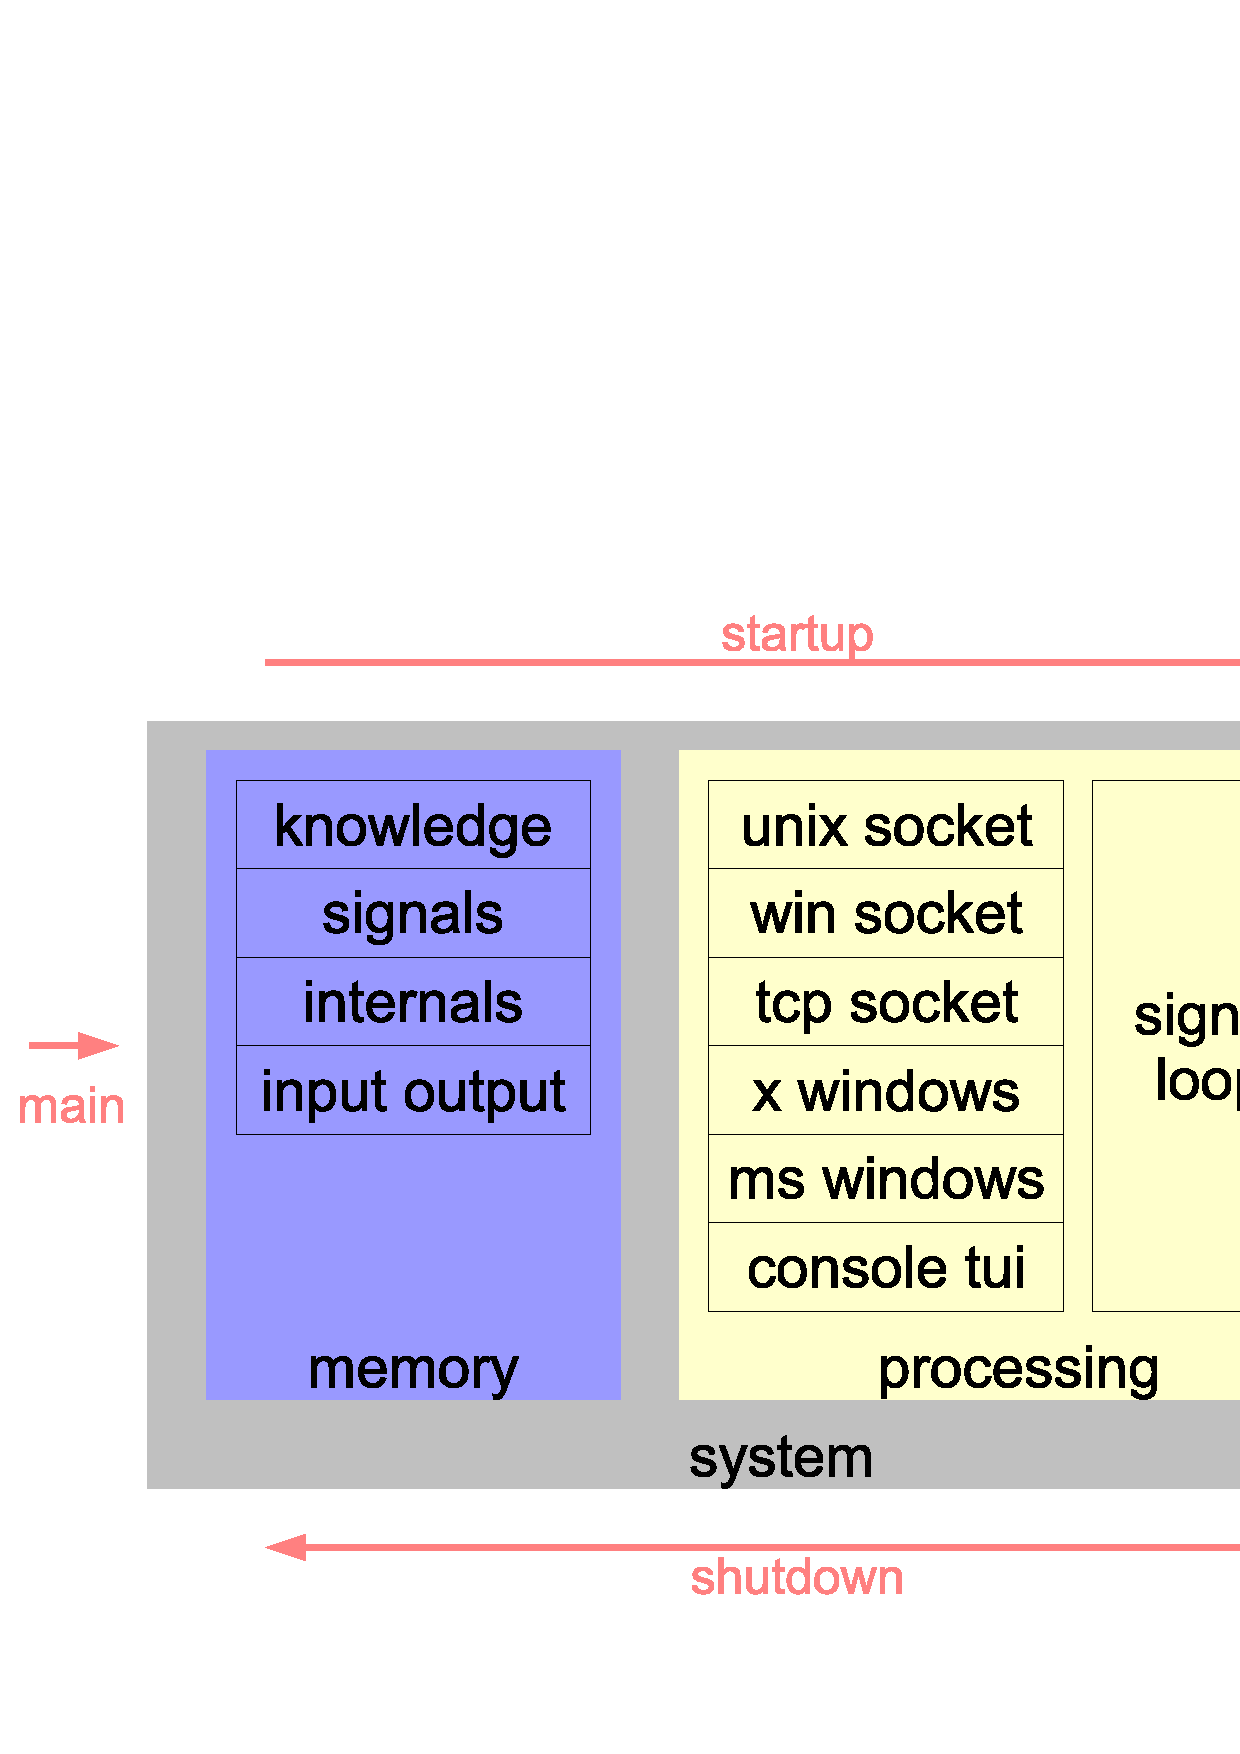
\includegraphics[scale=0.3,angle=-90]{graphic/system.pdf}
        \caption{System with Memory Structures, Processing Loops and Lifecycle}
        \label{system_figure}
    \end{center}
\end{figure}
